%
\chapter{Hilfsmittel/Arbeitsumgebung}
\label{chap:arbeit}

Zum Erstellen des Schaltplans und der Gerberfiles haben wir das auf den Laborrechnern bereitgestellte Tool Pulsonix verwendet.\\
Die Python Programmierung haben wir im Notepad++ durchgeführt.\\
Um den MSP430FR zu beschreiben griffen wir auf das vom Hersteller bereitgestellte Tool CCS zurück.

\subsection{Installation und anwendung des CCS}
\raggedright
Die aktuellste Version des CCS kann unter folgender URL bei ti direkt heruntergeladen werden \url{http://processors.wiki.ti.com/index.php/Download_CCS}.
Nach dem Ausführen der css\_setup.exe sollte im Schritt "processor support" wenigstens die Familie MSP430 wie in folgendem Screenshot gezeigt ausgewählt werden.\\
	\centering
	\fbox{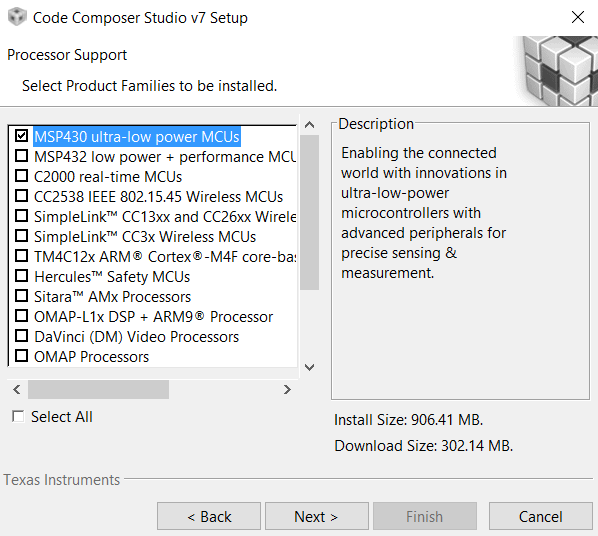
\includegraphics[width=0.5\textwidth]{media/ccs.PNG}}\\
\raggedright	
Nach der Installation des Programms kann ein Workspace angelegt oder ein bereits bestehender genutzt werden.
Beim Erstellen eines neuen Projektes sollte darauf geachtet werden, dass auch der richtige Microcontroller ausgewählt ist. Folgender Screenshot zeigt die korrekte Einstellung\\
	\centering
	\fbox{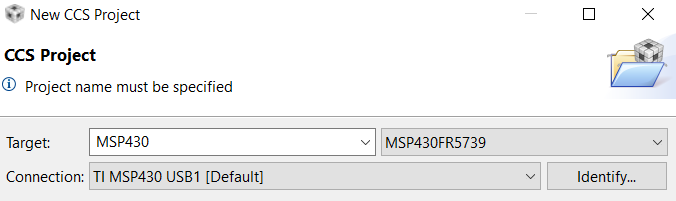
\includegraphics[width=0.5\textwidth]{media/ccs2.PNG}}\\
\raggedright	
Durch diese Auswahl werden bereits die richtigen Bibliotheken eingebunden.
Hier kann auch ein kleines Beispielprogramm erstellt werden, welches eine LED blinken lässt.
Die weitere Programmierung ist wie in herkömmlichen Entwicklungsumgebungen.
Eine nette und hilfreiche Erweiterung ist der Debugmodus, welcher uns schon oft weiter geholfen hat. Hier kann das Programm auf dem MSP430 direkt laufengelassen, angehalten und fortgesetzt werden.


Ein bereits fertiger Workspace-Ordner mit allen hier aufgelisteten Programme ist auch auf der CD zu finden.


\subsection{Erstellen des Download-Files}
Ein Programm, das mit dem MSP430Connect Skript auf den Mikrokontroller geladen werden soll muss in einem bestimmten Dateiformat vorliegen. Zur Erstellung dieser Datei müssen im Code Composer Studio (CCS) zuerst einige Einstellungen vorgenommen werden.

1. unter 'Build' Configuration auf Release stellen

2. unter 'MSP430 Hex Utility' haken bei Enable MSP430 Hex Utility aktivieren

3. unter 'Output Format Options' das Output format auf Output TI\_TXT hex Format setzen

4. Build Release ausführen, 'projektname'.txt liegt jetzt im workspace

Diese 'projektname'.txt muss dann dem MSP430Connect Skript als Parameter übergeben werden.